\documentclass[a4paper,11pt,twoside]{mgr}

%**************************************************************************
% Dane do strony tytułowej
%

% Autor
\autor{Dawid Ziora}

% Rodzaj pracy - wpisać LICENCJACKA, INŻYNIERSKA lub MAGISTERSKA
\rodzajPracy{INŻYNIERSKA}

% Tytuł pracy magisterskiej/inżynierskiej
\tytul{Aplikacja wspomagająca zarządzanie budżetem}

% Tytuł pracy magisterskiej w języku angielskim
\tytulAng{Application for Budget Management Support}

% Promotor
\promotor{dr inż. Bartosz Kowalczyk}

% Rok
\rok{2025}

% Kierunek
\kierunek{Informatyka}

% Studia stacjonarne lub niestacjonarne (wpisać jakie)
\studia{stacjonarne}

% Poziom studiów wpisać I lub II
\poziomStudiow{I}

% Numer albumu
\numerAlbumu{136700}

%
%**************************************************************************

% Styl dla wtrąceń anglojęzycznych
\newcommand{\eng}[1]{(\emph{#1})}
%\renewcommand{\baselinestretch}{1}
\renewcommand\lstlistlistingname{Spis listingów}

\begin{document}

\pagestyle{empty}
\stronaTytulowa
\cleardoublepage

\tableofcontents

\pagestyle{fancy}

\chapter{Wstęp}
Aplikacje webowe są coraz bardziej powszechnie używane. W artykule \cite{AcademyBank} zauważono, że 83.1\% osób śledzi swoje wydatki, z czego 45.3\% używa do tego narzędzi cyfrowych. Jednym z rozwiązań jest korzystanie z aplikacji budżetowych. W badaniach użycie tych narzędzi zadeklarowało 20.9\% ludzi. Z biegiem czasu te liczby będą tylko rosły, ponieważ na rynku będzie pojawiać się coraz więcej narzędzi umożliwiających proste zarządzanie własnymi finansami. Niemal 80\% osób korzystających z platform do zarządzania budżetem deklaruje, że korzysta z nich przynajmniej raz w tygodniu. 

W publikacji \cite{PFMApp} dowiadujemy się, że aplikacje te wpływają na wzrost wiedzy ekonomiczno-finansowej społeczeństwa, zwiększają chęć do planowania i kontroli budżetem domowym. Usługi te są dostępne w każdym miejscu i czasie 24/7. Przeprowadzone badanie na grupie $N=301$ polaków wykazało, że 288 korzysta z aplikacji do wspomagania budżetem, a tylko 13 nie korzysta. Główne czynności, do których Polacy wykorzystują aplikacje to Kontrola budżetu domowego (88.54\%), Weryfikacja wydatków z ostatniego miesiąca (86.11\%), Sprawdzanie salda rachunku/-ów (48.26\%) oraz planowanie wydatków na kilka miesięcy (45.83\%). 

Według artykułu \cite{FintechStats} grupą, która najczęściej używa tego typu aplikacji znajduje się w przedziale wiekowym od 27 do 42 lat. Około 91\% osób z tej grupy deklaruje użycie tego typu aplikacji. Kolejna grupa to osoby w wieku od 43-58 lat (80\%). W przedziale od 18 do 26 roku życia jest to 68\%. Według badań aktualna wielkość rynku wynosi około 441.47\$ miliardów i przy aktualnym tempie wzrostu może urosnąć nawet do 906\$ miliardów do 2029 roku.

Aplikacje te najczęściej cechują się interfejsem przyjaznym dla użytkownika, kategoryzacją i śledzeniem wydatków, możliwością przypominania o rachunkach oraz zapewniają ochronę informacji personalnych. Ich rozwój jest dynamiczny, na co wskazuje rosnąca liczba użytkowników.
\section{Cel pracy}
Celem pracy jest zbudowanie aplikacji do zarządzania budżetem użytkownika końcowego. Aplikacja ma za zadanie wspomagać użytkowników w kontroli wydatków, planowaniu budżetu oraz analizie danych finansowych w prosty sposób. 
\section{Zakres pracy}
Zakres niniejszej pracy obejmuje zaprojektowanie i implementację aplikacji webowej umożliwiającej zarządzanie budżetem domowym. 
Aplikacja została oparta na architekturze klient-serwer. 

Warstwa serwerowa została zaimplementowana w języku Java z wykorzystaniem frameworka Spring Boot. Wykorzystana została 21 wersja JAVY. Zapewnia obsługę logiki biznesowej, komunikację z bazą danych oraz interfejs API w technologii REST.  Korzysta między innymi z takich zależności jak: 
\begin{itemize}
	\item Lombok - Ułatwia tworzenie klas i podstawowych funkcji w klasach.
	\item DevTools - Pozwalające m.in. na przeładowanie w czasie rzeczywistym.
	\item Web - Zawiera RESTful API, pozwala na komunikacje.
	\item Security - Umożliwia zastosowanie zabezpieczeń i autoryzacji do kontrolowania aplikacji.
	\item MongoDB - Do przechowywania dokumentów w formacie zbliżonym do JSON.
	\item Validation - pozwala na walidacje pól na przykład: ustawienie długości pola, pole nie może być puste i tym podobne.
\end{itemize}
Testy jednostkowe są wykonywane przy pomocy biblioteki JUnit w wersji 5. Testy są wykonywane przed uruchomieniem aplikacji, aby sprawdzić jej poprawne działanie. 

Warstwa frontendowa została zrealizowana w oparciu o React + Vite. Język, wykorzystany po stronie frontendu to TypeScript, który jest językiem skupiającym się silnie na typach danych. Pozwala to na dokładne określenie wyświetlanych na stronie informacji. Elementy, z których zbudowana jest strona są wykorzystane z popularnego reactowego frameworka UI o naziwe Ant Design. Składa się on ze wstępnie zbudowanych komponentów, które łatwo jest wyświetlić na stronie internetowej.

Dane są przechowywane w nierelacyjnej bazie danych MongoDB, która zawiera dokumenty JSON ze wszystkimi ważnymi informacjami, które są związane z użytkownikami aplikacji.


W ramach projektu utworzone są funkcje takie jak:
\begin{itemize}
	\item Rejestracja - Pozwala na utworzenie nowego konta przez użytkownika
	\item Logowanie - Umożliwia dostęp do konta oraz funkcji strony
	\item Tworzenie transakcji - Zapewnia możliwość dokonywania przelewów, wpłat i wypłat z konta
	\item Wizualizacja danych na wykresie
\end{itemize}
Do sprawdzenia poprawności działania tych i innych funkcji wykorzystuje się narzędzie Postman, które pozwala wysyłać zapytania, sprawdzać restpointy i ogólną komunikację między klientem a serwerem. Narzędzie to jest powszechnie wykorzystywane przez deweloperów, ponieważ ułatwia ich pracę i umożliwia szybszy sposób na sprawdzanie poprawności działania funkcji bez konieczności implementacji ich na stronie internetowej. 

Aplikacja wykorzystuje tez konteneryzacja, czyli jest zapakowane w wirtualny kontener na którym są wykonywane wszystkie operację. Do tego celu służy silnik Docker Engine, który umożliwia pobieranie wirtualnych obrazów systemów. Pozwala to na automatyzację pracy oraz niezmienność wersji programu w procesie wytwarzania oprogramowania. Daje możliwość, by daną aplikację uruchomić na dowolnym komputerze, bez konieczności posiadania zainstalowanych aplikacji takich jak mongoDB, wirtualnej maszyny Javy, czy też menadżera pakietów npm.


\section{Struktura pracy (Budowa pracy)}
Streszczenie wszystkiego (1 akapit) - bez wstępu 

W pierwszym rozdziale zostały opisany wszystkie technologię oraz narzędzia użyte do uzyskania działającej aplikacji. Znajdują się w niej najważniejsze informacje o każdej z nich oraz pojedyncze przykłady ich zastosowań.

Drugi rozdział skupia się na wymaganiach postawionych projektowi. Przedstawia również diagramy na których możemy zobaczyć w jaki sposób mają działać funkcję.

Trzeci rozdział uwzględnia informacje o tym w jaki sposób został utworzony cały projekt. Tłumaczy w jak działają poszczególne technologie, narzędzia i opisuje całą aplikację.

W czwartym rozdziale znajdują się informacje o tym jak użytkownik powinien korzystać ze strony. Jest to instrukcja dla użytkownika, aby mógł zrozumieć, gdzie należy szukać odpowiednich elementów strony. Przedstawia krótkie opisy wraz z obrazkami. 

Piąty rozdział zawiera podsumowanie całej pracy. Zostały w nim wyciągnięte wnioski oraz moje osiągnięcia.

\chapter{Przegląd technologii stosowanych w aplikacjach klient-serwer}
W procesie wytwarzania oprogramowania częstym problemem jest wybór odpowiednich rozwiązań, które pozwolą nam w najlepszy sposób osiągnąć zamierzone cele. Znajomość kompatybilnych technologii w znaczącym stopniu przyśpiesza tworzenie aplikacji webowych. Projekt można podzielić na warstwę prezentacji, która odpowiada za interfejs graficzny oraz interakcję z użytkownikiem, warstwę serwerową odpowiadającą za logikę biznesową aplikacji oraz komunikację z bazą danych oraz warstwę dostępu do danych, która odpowiada za trwałe przechowywanie rekordów i ich udostępnianie innym warstwą.
\section{Architektura systemu}
Jednym ze sposobów projektowania aplikacji sieciowych jest model klient-serwer. Klient nie posiada danych oraz funkcji, dlatego musi kontaktować się z programem posiadającym dostęp do danych oraz usług. Program ten nazywany jest serwerem. 

Klient zleca serwerowi żądanie pewnej usługi, następnie serwer analizuje polecenia i wysyła odpowiedź. Model ten jest powszechnie używany w aplikacjach dostępnych za pośrednictwem internetu \cite{ArchKS}. 

\subsection*{Przykładowe zastosowanie w aplikacji webowej}
Próba logowania na stronę WWW jest równoważna z wysłaniem do serwera wiadomości z typem operacji, oraz podanymi w formularzu wartościami. Serwer otrzymując taką wiadomość wykonuje niezbędne testy na przykład: sprawdza poprawność otrzymanych danych. Po pomyślnym dokonaniu sprawdzeń serwer wykonuje żądaną operację i wysyła odpowiedź klientowi \cite{ArchKS}.

\subsection*{Kody odpowiedzi HTTP}
Odpowiedź serwera to numeryczna dana wysłana przez serwer, która ma na celu poinformowanie użytkownika o realizacji pewnego zadania. Kody dzielą się na informacyjne, które zaczynają się od 1xx, powodzenia zaczynające się od 2xx, przekierowania (3xx), błędu aplikacji klienta (4xx), błędu serwera HTTP (5xx) \cite{TempWiki}.
\begin{table}[H]
	\centering
	\caption{Przykładowe opisy odpowiedzi serwera}
	\begin{tabular}{|c|p{2cm}|p{10cm}|}
		\hline
		\textbf{Kod} & \textbf{Opis słowny} & \textbf{Znaczenie} \\ \hline
		100 & Continue & Prośba o dalsze wysłanie zapytania \\ \hline
		200 & OK & Zawartość żądania (najczęściej zwracany nagłówek)\\ \hline
		201 & Created & Wysłany dokument został zapisany na serwerze \\ \hline
		204 & No content & Serwer nie potrzebuje zwracać żadnej treści \\ \hline
		300 & Multiple Choices & Istnieje więcej niż jeden sposób obsłużenia danego zapytania \\ \hline
		302 & Found & Zasób jest chwilowo dostępny pod innym adresem \\ \hline
		400 & Bad Request & Żądanie nie może być obsłużone przez serwer z powodu nieprawidłowości postrzeganej jako błąd użytkownika \\ \hline
		401 & Unauthorized & Żądanie zasobu, który wymaga uwierzytelnienia \\ \hline
		403 & Forbidden & Serwer zrozumiał zapytanie, jednak konfiguracja bezpieczeństwa zabrana mu zwrócić żądany zasób \\ \hline
		404 & Not Found & Serwer nie znalazł zasobu według podanego adresu URL\\ \hline
		500 & Internal Server Error & Serwer napotkał niespodziewane trudności \\ \hline
		502 & Bad Gateway & Serwer spełniający rolę bramy otrzymał niepoprawną odpowiedź od serwera nadrzędnego \\ \hline
		503 & Service Unavaiable & Serwer nie jest w stanie zrealizować żądania użytkownika ze względu na przeciążenia \\ \hline
		504 & Gateway Timeout & Serwer spełniający rolę bramy nie otrzymał odpowiedzi w ustalonym czasie \\ \hline
	\end{tabular}
\end{table}

\begin{figure}[H]
	\centering
	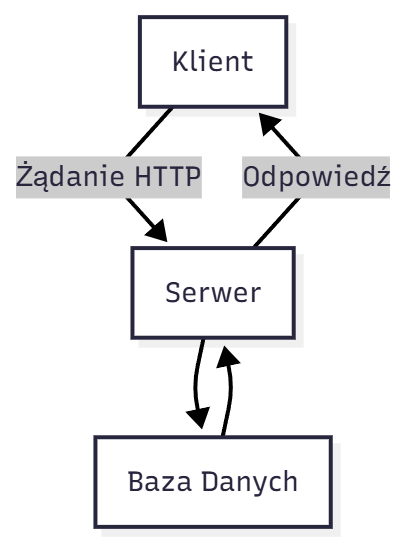
\includegraphics[width=0.4\textwidth]{images/Klient-Serwer.png}
	\caption{Diagram przedstawiający architekturę klient-serwer}
	\label{fig:KlientSerwer}
\end{figure}
\section{Java}
Java jest obiektowym wieloplatformowym językiem programowania. Jest ona jednym z najpopularniejszych języków dla deweloperów oprogramowania \cite{JavaMicrosoft}. Korzysta z wirtualnej maszyny Java (JVM), które mogą zostać zainstalowane na większości komputerów i urządzeń przenośnych. Został on stworzony z myślą ,,napisz raz, uruchamiaj w dowolnym miejscu''. 
\\W projekcie jest odpowiedzialny za logikę biznesową aplikacji, przetwarzanie danych oraz komunikację z bazą danych \cite{JDK21Docs}.
\subsection*{Spring Boot}
Framework Spring Boot pozwala znacząco uprościć proces tworzenia aplikacji webowej w Javie. Eliminuje konieczność ręcznej konfiguracji wielu elementów. Pełni on role fundamentu dla warstwy serwerowej, udostępniając interfejs REST API, który umożliwia komunikację przy użyciu odpowiednich punktów końcowych (ang. \textit{endpoints}). Składa się z takich rzeczy jak:
\begin{itemize}
	\item Controller - obsługuje żądania HTML
	\item Repository - odpowiada za komunikacje z bazą danych
	\item Config - Obejmuje konfiguracje aplikacji, polityki bezpieczeństwa, ciasteczka
	\item Model - Reprezentuje dane w postaci klas, które są odwzorowaniem tabel w bazie danych.
	\item Resource - Znajdują się w nim właściwości aplikacji, oraz statyczne elementy.
\end{itemize}
Spring Boot wspiera również takie mechanizmy jak Wstrzykiwanie zależności (ang. \textit{Dependency Injection}) oraz AOP (ang. \textit{Aspect-Oriented Programming}) \cite{SpringDocs}.
\subsection*{Maven}
W projekcie wykorzystano narzędzie Apache Maven, które pełni role automatyzacji budowy i zarządzania zależnościami. Pozwala zdefiniować wszystkie wymagane biblioteki i frameworki w jednym centralnym pliku pom.xml (ang. Project Object Model). Działa w oparciu o repozytoria, w których przechowywane są biblioteki. Główny plik zawiera takie informacje jak:
\begin{itemize}
	\item groupId, artifactId, version - identyfikatory projektu,
	\item sekcję dependencies - listę bibliotek, które mają zostać automatycznie pobrane,
	\item sekcję build - ustawienia dotyczące budowania aplikacji,
	\item sekcje plugins - narzędzia wspierające proces budowania
\end{itemize}
W przypadku aplikacji opartej na Spring Boot, Maven pobiera również tzw. startery np.:
\begin{itemize}
	\item spring-boot-starter-web - uruchamia aplikacje serwerową (np. Tomcat) i pozwala tworzyć kontrolery REST
	\item spring-boot-starter-data-mongodb - Umożliwia korzystanie z bazy mongo
	\item spring-boot-starter-security - Dodaje mechanizmy autoryzacji i uwierzytelniania
	\item spring-boot-starter-test - pozwala na testowanie aplikacji
\end{itemize}
Cała konfiguracja środowiska sprowadza się do utworzenia odpowiedniego pliku z zależnościami, a Spring Boot automatycznie na jego podstawie konfiguruje je przy uruchomieniu \cite{MavenDocs}.
\subsubsection*{Dane do wstawienia w ten rozdział}
 Korzysta między innymi z takich zależności jak: 
\begin{itemize}
	\item Lombok - Ułatwia tworzenie klas i podstawowych funkcji w klasach.
	\item DevTools - Pozwalające m.in. na przeładowanie w czasie rzeczywistym.
	\item Web - Zawiera RESTful API, pozwala na komunikacje.
	\item Security - Umożliwia zastosowanie zabezpieczeń i autoryzacji do kontrolowania aplikacji.
	\item MongoDB - Do przechowywania dokumentów w formacie zbliżonym do JSON.
	\item Validation - pozwala na walidacje pól na przykład: ustawienie długości pola, pole nie może być puste i tym podobne.
\end{itemize}
\section{React}
React to jedna z bibliotek JavaScript służąca do tworzenia interfejsów użytkownika (ang. User Interface) w aplikacjach webowych. Jest oparta na koncepcji komponentów, które można łatwo ze sobą łączyć i w czytelny sposób wyświetlać na stronie. React pozwala renderować widoki na podstawie mechanizmu Virtual DOM (ang. Document Object Model). Obiekt DOM umożliwia dostęp do struktury strony w celu jej modyfikacji. W przypadku modelu wirtualnego minimalizuje operacje na drzewie rzeczywistym. 
\subsection*{Vite}
W celu usprawnienia procesu tworzenia aplikacji zastosowano narzędzie Vite, które pełni rolę bundlera, czyli łączy ze sobą wiele plików m.in. kody źródłowe i zależności. Rozwiązanie to oferuje szybkie uruchamianie środowiska, optymalizacja kodu i co najważniejsze w usprawnieniu pracy poprzez przeładowanie kodu na bieżąco (ang. Hot Module Replacement), który pozwala wyświetlać zmiany bez konieczności ponownego budowania całej aplikacji. 
\subsection*{TypeScript}
Komponenty oraz wszystkie składowe projektu są przygotowane w języku TypeScript, który jest nadzbiorem języka JavaScript. Wprowadza on statyczne typowanie, znaczy to że typy są określone i sprawdzane w czasie kompilacji. Pozwala wprowadzać typy dla zmiennych, funkcji i obiektów. Dzięki temu kod jest bardziej czytelny i zrozumiały dla developera. 
\newline

Połączenie Reacta, Vite oraz TypeScript zapewnia wydajne i przyjemne środowisko dla pracy programisty, lepszą kontrole nad danymi i wydajność pracy. Technologie te zostały wybrane również dla bogatego wyboru bibliotek wspieranych przez react. Jedną z nich jest biblioteka AntD, która zawiera wstępnie przygotowane do użycia na stronie komponenty. 

\section{MongoDB}
MongoDB to nierelacyjna baza typu NoSQL. W przeciwieństwie do klasycznych baz relacyjnych MongoDB nie korzysta z tabel, lecz przechowuje dane w postaci dokumentów BSON (Binary JSON), które strukturą przypominają obiekty JSON.
Jeden dokument może mieć wiele różnych pól, co pozwala bardziej elastycznie modelować dane. Baza ta korzysta z kolekcji (ang. collections), które są odpowiednikami tabel w klasycznych bazach relacyjnych. Każdy wpis w bazie posiada własny unikatowy identyfikator \_id. Wspiera ona wiele operacji, takich jak sortowanie, filtrowanie, czy grupowanie. Zaimplementowanie ich w kodzie programu jest proste i wystarczy do tego odpowiednio utworzone repozytorium z odpowiednimi operacjami (lst. \ref{lst:java-repo}). Połączenie bazy w aplikacji Java odbywa się za pomocą modułu Spring Data MongoDB. To właśnie ten moduł odpowiada za możliwość tworzenia repozytorium.
\begin{lstlisting}[language={Java}, caption={Przykładowe repozytorium w Javie}, label={lst:java-repo}]
@RepositoryRestResource(collectionResourceRel = "users", path = "users")
public interface UserRepository extends MongoRepository<User, String> {
	Optional<User> findByLogin(String login);
	List<User> findByLoginContainingIgnoreCase(String loginPart);	
}	
\end{lstlisting}
Powyższy fragment kodu pozwala znaleźć użytkownika po loginie lub wyszukać wszystkich użytkowników zawierających podany ciąg znaków w swojej nazwie.
\begin{lstlisting}[caption={Przykladowy dokument z kolekcji}, label={lst:MongoDB-doc}]
{
	"id": "68d56ad95a544e07c8ebaa54",
	"login": "ADMIN",
	"password": "$2a$10$.itTB4jFiMBPdZSDebVE4Obtl8FpDiT7CHovqCtq8dcUnFMoe1gem",
	"role": "ADMIN"
}
\end{lstlisting}

\chapter{Architektura aplikacji}
W rozdziale przedstawiono wymagania funkcjonalne i niefunkcjonalne, które zostały postawione aplikacji. Zaprezentowano również diagramy przypadków użycia, stanów oraz sekwencji.
\section{wymagania funkcjonalne}
Wymagania funkcjonalne określają zachowanie systemu i jego reakcji na określone zadania \cite{Wymagania}.
\begin{table}[!h]
	\centering
	\renewcommand{\arraystretch}{1.3}
	\setlength{\tabcolsep}{6pt}
	\begin{tabular}{|c|p{5cm}|p{8cm}|}
		\hline
		\textbf{Nr} & \textbf{Wymaganie funkcjonalne} & \textbf{Opis} \\ \hline
		
		1. & Rejestracja użytkownika & System umożliwia utworzenie konta użytkownika z danymi logowania. \\ \hline
		2. & Logowanie do systemu & System weryfikuje dane użytkownika i umożliwia dostęp do panelu aplikacji. \\ \hline
		3. & Sprawdzenie dostępnych środków & Użytkownik może sprawdzić ile posiada balansu na koncie. \\ \hline
		4. & Wpłata pieniędzy na konto & Użytkownik może zasilić konto. \\ \hline
		5. & Przegląd historii wydatków & Aplikacja wyświetla listę wszystkich wydatków. \\ \hline
		6. & Tworzenie przelewu & System pozwala stworzyć przelew użytkownikowi. \\ \hline
		7. & Podsumowanie finansów konta & Użytkownik może sprawdzić dane o swoich wydatkach dla danego konta. \\ \hline
		8. & Kategoryzowanie transakcji & Użytkownik może podać kategorię dla wpłat i wypłat z konta. \\ \hline
		9. & Prezentacja wydatków na wykresie & System wyświetla wykres z wydatkami za dzień, tydzień, miesiąc oraz rok. \\ \hline
	\end{tabular}
	\caption{Wymagania funkcjonalne systemu do zarządzania budżetem domowym}
	\label{tab:wymagania_funkcjonalne}
\end{table}

\section{Wymagania niefunkcjonalne}
Wymaganiami funkcjonalnymi nazywamy wszystkie potrzeby, które nie dotyczą funkcjonalności produktu \cite{Wymagania}. Wymagania te opisują m.in. jak szybko system powinien odpowiadać na żądania, w jakim czasie produkt ma zostać dostarczony, jak ma prezentować się interfejs użytkownika. 
\begin{table}[H]
	\centering
	\renewcommand{\arraystretch}{1.3}
	\setlength{\tabcolsep}{6pt}
	\begin{tabular}{|c|p{3.1cm}|p{9.9cm}|}
		\hline
		\textbf{Nr} & \textbf{Wymaganie niefunkcjonalne} & \textbf{Opis} \\ \hline
		
		1. & Niezawodność & System w krótkim czasie odzyskuje pełną funkcjonalność w przypadku wystąpienia błędu. \\ \hline
		2. & Dostępność & System ma być dostępna przez 99.5\% czasu działania serwera.\\ \hline
		3. & Wydajność & System reaguje na żądanie w czasie krótszym niż 1 sekunda. Może obsłużyć do 1000 użytkowników jednocześnie. System jest w stanie przetworzyć do 10 GB na godzinę.  System jest skalowalny.\\ \hline
		4. & Bezpieczeństwo & System zapewnia, że dane są dostępne tylko dla osób upoważnionych. Autoryzacja użytkowników odbywa się poprzez podanie odpowiedniego loginu oraz hasła. Hasła muszą być przechowywane w formie zaszyfrowanej. \\ \hline
		5. & Wdrożenie & Aplikacja serwerowa musi być uruchomiona w środowisku JVM oraz korzystać z wersji Java 21 , Warstwa prezentacji uruchamiana w środowisku NodeJs z wykorzystaniem 9 wersji biblioteki React. Dane przechowywane w postaci dokumentów bazy danych MongoDB w wersji 8, Aplikacja uruchomiana jest w środowisku systemu operacyjnego Windows 11 oraz Linux \\ \hline
		
	\end{tabular}
	\caption{Wymagania niefunkcjonalne systemu do zarządzania budżetem domowym}
	\label{tab:wymagania_niefunkcjonalne}
\end{table}
\section{Diagramy przypadków użycia}
Diagram przypadków użycia (ang. \textit{Use Case Diagram})
\begin{figure}[H]
	\centering
	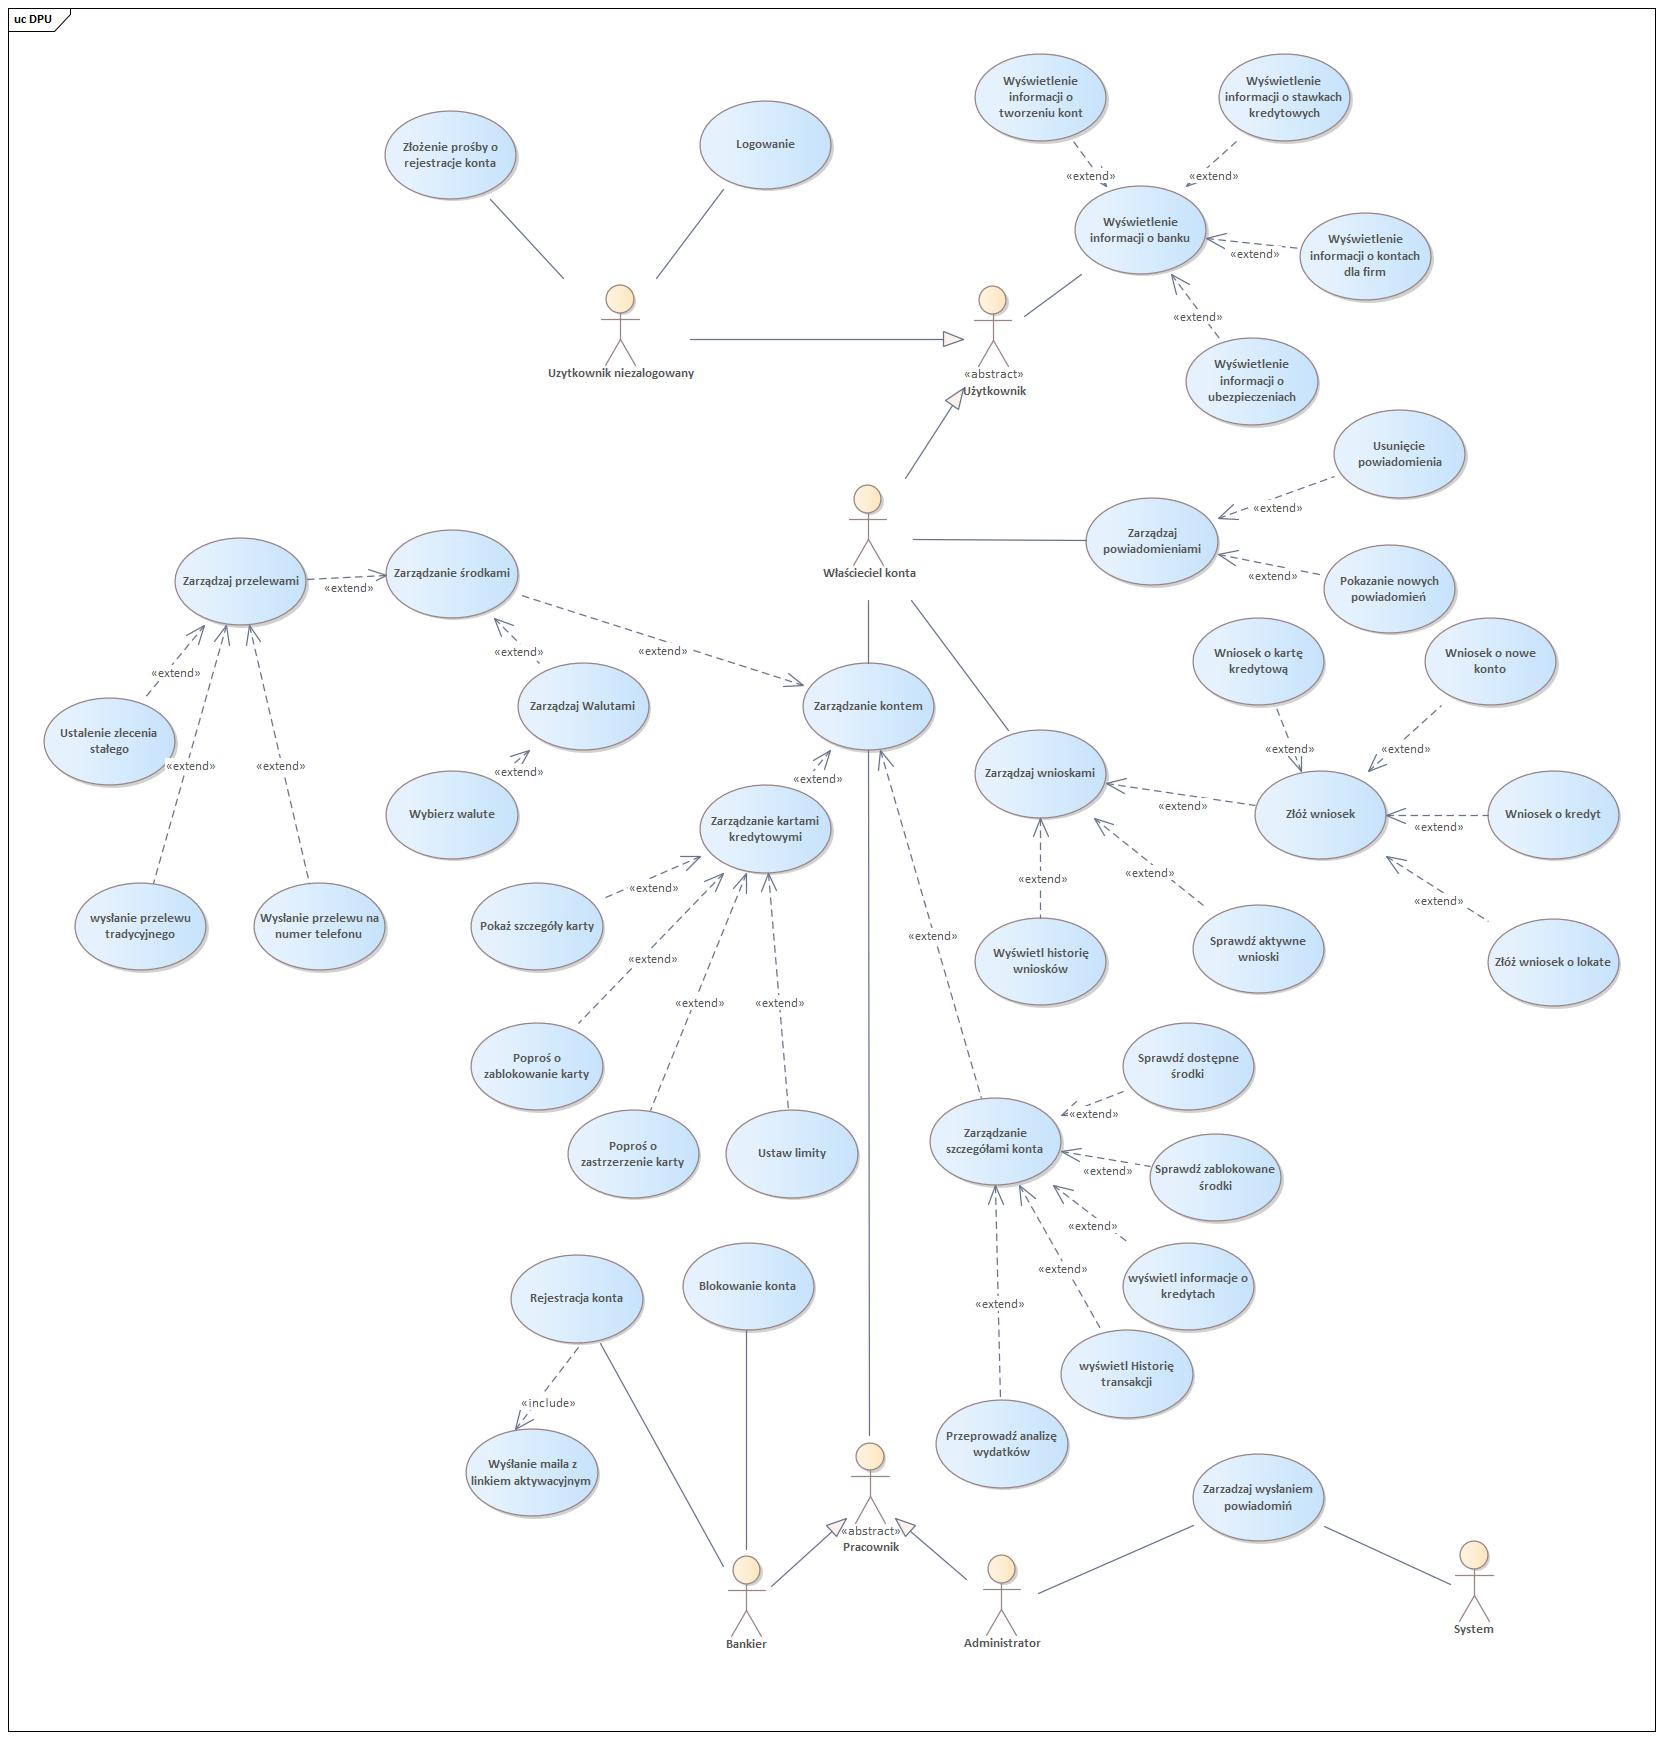
\includegraphics[width=1\textwidth]{images/DPU.jpg}
	\caption{Diagram przypadków użycia}
	\label{fig:UseCase}
\end{figure}
\section{Diagram stanów}
\begin{figure}[H]
	\centering
	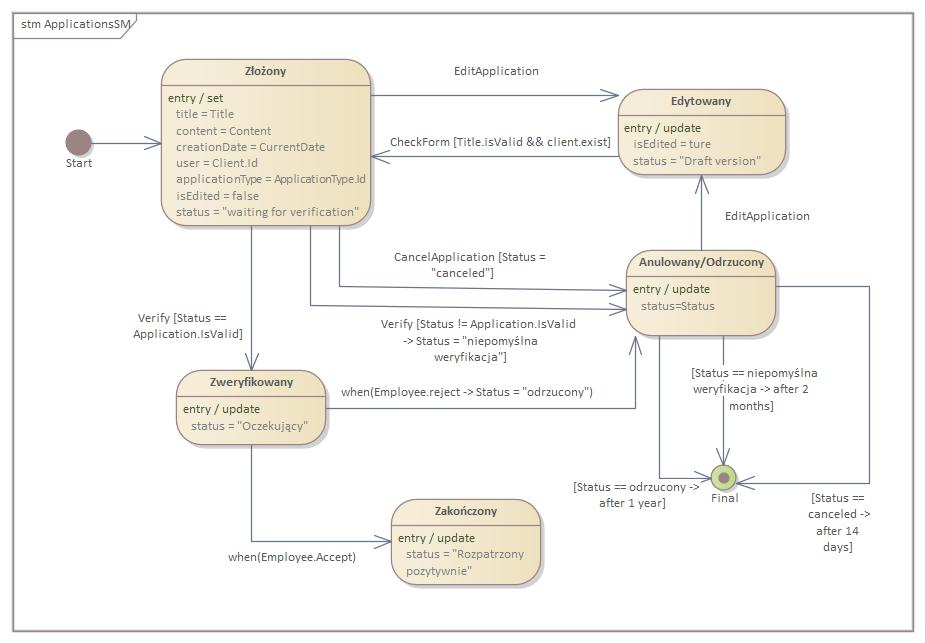
\includegraphics[width=1\textwidth]{images/Wniosek.jpg}
	\caption{Diagram stanów składania wniosku}
	\label{fig:StateMachine}
\end{figure}
\section{Diagramy sekwencji}
\begin{figure}[H]
	\centering
	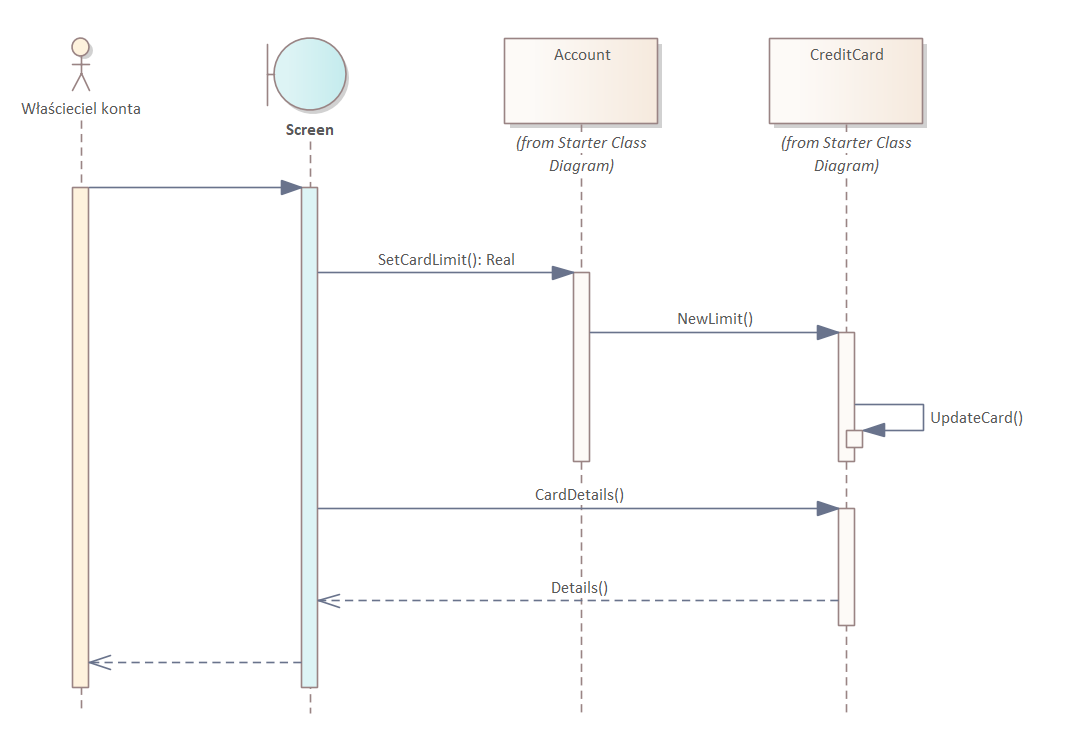
\includegraphics[width=0.7\textwidth]{images/Limit.png}
	\caption{Diagram sekwencji Limit}
	\label{fig:Seq1}
\end{figure}
\begin{figure}[H]
	\centering
	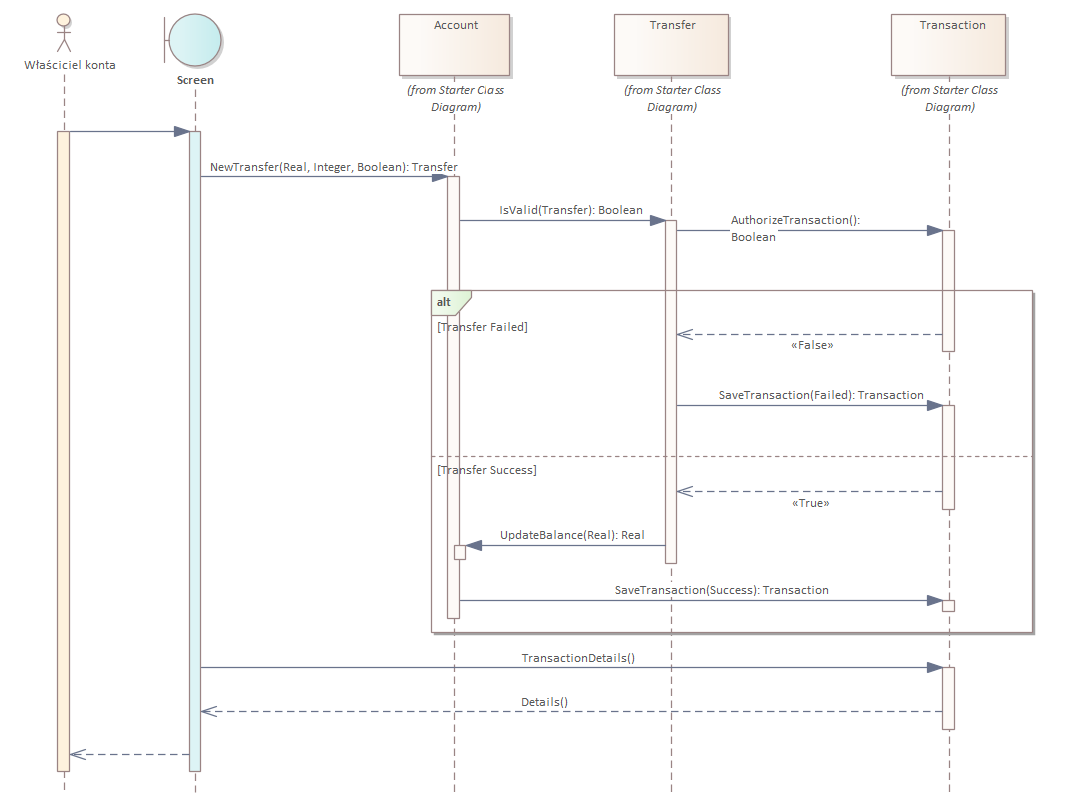
\includegraphics[width=0.7\textwidth]{images/Przelew.png}
	\caption{Diagram sekwencji Przelew}
	\label{fig:Seq2}
\end{figure}
\chapter{Implementacja systemu}
Rozdział  przedstawia proces implementacji systemu. Omówiono w nim wykorzystane technologie oraz poszczególne warstwy aplikacji. Celem tego rozdziału jest zaprezentowanie działania wykorzystanej architektury oraz korelacje między poszczególnymi elementami systemu.
\section{Backend – logika biznesowa i API}
Warstwa serwerowa odpowiada ze przetwarzanie żądań od warstwy prezentacji oraz za komunikację z bazą danych. Elementy z których jest skonstruowana to m.in. kontrolery, repozytoria, czy pliki konfiguracyjne. Została zrealizowana w oparciu o framework Spring Boot, który upraszcza proces tworzenia aplikacji dzięki zestawowi tzw. starterów.

\subsection*{Spring Boot i ekosystem bibliotek}
Freamework spring boot oferuje moduły oraz biblioteki wykorzystane do budowy REST API, dostępu do baz danych, bezpieczeństwa i testowania. Wykorzystywane biblioteki są deklarowane w pliku \texttt{pom.xml}. Są one wstępnie skonfigurowane. Takie rozwiązanie znacząco zwiększa tępo rozwoju aplikacji, pozwala na lepszą pracę w grupach oraz redukuje ilość kodu szablonowego (ang. \textit{boilerplate code}).
\subsubsection*{Zarządzanie zależnościami i startery}
Spring boot łączy biblioteki w postaci starterów. Pozwala to zminimalizować ryzyko konfliktów wersji oraz skrócić czas konfiguracji. Kluczowe startery wykorzystywane w aplikacji webowej to:
\begin{itemize}
	\item \textbf{spring-boot-starter-web} -- Warstwa HTTP/REST oparta na spring MVC, która udostępnia wbudowany serwer Tomcat. 
	\item \textbf{spring-boot-starter-data-jpa} -- Umożliwia dostęp do relacyjnej bazy danych poprzez JPA (ang. \textit{Java Persistence API}).
	\item \textbf{spring-boot-starter-data-mongodb} -- Pozwala na dostęp do nierelacyjnej bazy MongoDB. 
	\item \textbf{spring-boot-starter-validation} -- Implementuje biblioteki do walidacji danych wejściowych.
	\item \textbf{spring-boot-starter-security} -- Mechanizm uwierzytelniania, autoryzacji i ochrony endpointów.
	\item \textbf{spring-boot-starter-test} -- Środowisko testowe do testów jednostkowych i integracyjnych. 
	\item \textbf{Lombok} -- Redukuje kod szablonowy (gettery, settery, konstruktory).
\end{itemize}
\subsubsection*{Warstwa webowa}
Umożliwia komunikację z wykorzystywaniem standardu REST API (ang. \textit{Representational State Transfer Application Programing Interface}). W warstwie kontrolerów tworzone są endpointy w oparciu o modele z jakimi są związane. Kontroler może implementować obsługę żądań HTTP, takich jak:
\begin{itemize}
	\item POST -- Przesyłanie danych na serwer
	\item GET -- Pobieranie danych z serwera
	\item PUT -- Aktualizowanie danych na serwerze
	\item DELETE -- Usuwanie danych z serwera
\end{itemize}
Mapowanie endpointów w kontrolerze jest pokazane w listingu \ref{lst:java-endpoints}.
\begin{lstlisting}[language={Java}, caption={Przykładowe Endpointy}, label={lst:java-endpoints}]
@RestController 
@RequestMapping("/User") // Wszystkie endpointy zaczynają się od /User
	@PostMapping("/register")		// Dostęp pod POST /User/register
	@GetMapping("/search")			// Dostęp pod GET /User/search
	@PutMapping("/update/{id}")		// Dostęp pod PUT /User/update/{id}
	@DeleteMapping("/delete/{id}")	// Dostęp pod DELETE /User/delete{id}
\end{lstlisting}

Implementacja powyższych endpointów znajduje się w listingach (\ref{lst:java-register}, \ref{lst:java-list}, \ref{lst:java-delete}, \ref{lst:java-update})
\subsubsection*{Dostęp do danych}
Połączenie z bazą danych zostało zrealizowane z wykorzystaniem \\ \texttt{spring-boot-starter-data-mongodb}, który udostępnia spójny model pracy z dokumentową bazą MongoDB. Pozwala mapować obiekty klas na dokumenty i tworzyć repozytoria oparte na interfejsach.

Utworzenie klasy mapowanej do dokumentu wymaga oznaczenia adnotacją \texttt{@Document}, a klucza głównego \texttt{@Id}. Identyfikator przeważnie określa się typem String (listing \ref{lst:java-Account}). 

Warstwa repozytoriów opiera się na interfejsach rozszerzających \texttt{MongoRepository<T, ID>}. Repozytoria pozwalają na podstawie nazw generować implementację metod wyszukujących (listing \ref{lst:java-Repository}).
\begin{lstlisting}[language={Java}, caption={Fragment modelu Account}, label={lst:java-Account}]
@Document
public class Account {
	@Id
	private String id;
	private String name;
	@Size(min = 25, max = 25)
	@Indexed(unique = true)
	private String number;
	private Currency currency;
	private String userId;
	...
\end{lstlisting}
\begin{lstlisting}[language={Java}, caption={Repozytorium dla klasy Account}, label={lst:java-Repository}]
@RepositoryRestResource
public interface AccountRepository extends MongoRepository<Account, String> {
	List<Account> findByUserId(String userId);
	Optional<Account> findByNumber(String number);
}
	\end{lstlisting}
\subsubsection*{Bezpieczeństwo}
Spring Security zapewnia mechanizm uwierzytelniania JWT (ang. \textit{JSON Web Token}) i filtrowania żądań. Token umożliwia autoryzowane połączenie z serwerem dzięki mechanizmowi ciasteczek. Token bezpieczeństwa składa się z trzech części (tab. \ref{tab:JWT}), które zwyczajowo wyglądają w następujący sposób \texttt{xxxxx.yyyyy.zzzzz}. Filtrowanie pozwala m.in. na określenie żądań, które mogą zostać wykonane bez konieczności autoryzacji użytkownika.

\begin{longtable}{|p{3cm}|p{5cm}|p{6cm}|}
		\caption{Struktura tokenu JWT \cite{JWT}}
		\label{tab:JWT} \\
\hline
\textbf{Nawza} & \textbf{struktura} & \textbf{Opis} \\ \hline

Nagłówek (ang. \textit{Header}) &
 \texttt{\{} \newline
 \hspace*{1em}\texttt{"alg": "HS256",} \newline
 \hspace*{1em}\texttt{"typ": "JWT"} \newline
 \texttt{\}} & 
 Nagłówek składa się z wykorzystanego algorytmu oraz z typu użytego tokena. \\ \hline
 Ładunek (ang. \textit{Payload}) &
  \texttt{\{} \newline
 \hspace*{1em}\texttt{"sub": "1234567890",} \newline
 \hspace*{1em}\texttt{"name": "John Doe"} \newline
 \hspace*{1em}\texttt{"admin": "true"} \newline
 \texttt{\}} & 
 Ładunek zawiera roszczenia (ang. \textit{claims}), czyli oświadczenia dotyczące podmiotu i dodatkowe dane. Typy roszczeń to: rejestrowane (ang. \textit{registered}), publiczne (ang. \textit{public}) i prywatne (ang. \textit{private}).
 \\ \hline
  Podpis (ang. \textit{Signature}) &
\texttt{HMACSHA256(} \newline
 \hspace*{1em}\texttt{base64UrlEncode(header)} \newline
 \hspace*{1em}\texttt{+ "."\space +} \newline
 \hspace*{1em}\texttt{base64UrlEncode(payload)} \newline
 \hspace*{1em}\texttt{, secretPassword)} &
  Podpis składa się z zaszyfrowanego nagłówka, ładunku i hasła, które są później przetwarzane przez wybrany algorytm. 
 \\ \hline

\end{longtable}

\subsubsection*{Testowanie}
Narzędzia do wykonywania testów dostarcza \texttt{spring-boot-starter-test}. Testy jednostkowe wykonuje się z wykorzystaniem biblioteki JUnit. Polegają na wysłaniu żądania HTTP do serwera i porównaniu odpowiedzi otrzymanej z oczekiwaną (przykładowe kody odpowiedzi w tabeli \ref{tab:Kody-HTTP}). W testach tego typu ważną cechą jest sprawdzenie wartości granicznych (listing \ref{lst:java-UnitTest}). 

Testy integracyjne pozwalają sprawdzić interakcje między komponentami aplikacji dzięki narzędziu MockMVC.
\subsubsection*{Konfiguracja i uruchamianie}
Konfiguracja środowiska odbywa się w pliku \texttt{application.properties}. Definicja plików \texttt{Dockerfile} oraz \texttt{Docker-compose.yml} pozwala na spójne uruchamianie usług w różnych środowiskach.
\subsection*{Przykładowe fragmenty kodu}
\subsubsection*{rejestracja}
Funkcja rejestracji przyjmuje jako argument obiekt klasy User, który posiada poprawnie uzupełnione ciało (login: String, password: String, role: UserRoles). Jeżeli podane dane są poprawne, zostaje wywołana funkcja szyfrująca hasło, a następnie użytkownik jest zapisywany w bazie danych.
\begin{lstlisting}[language={Java}, caption={Rejestracja użytkownika}, label={lst:java-register}]
@PostMapping("/register")
public String register(@Valid @RequestBody User user) {
	user.setPassword(passwordEncoder.encode(user.getPassword()));
	userRepository.insert(user);
	return "Rejestracja udana";
}
\end{lstlisting}
\subsubsection*{Lista użytkowników}
Funkcja \texttt{getUser()} wykorzystuję metodę z repozytorium, która umożliwia pobranie wszystkich dokumentów i zwraca je.
\begin{lstlisting}[language={Java}, caption={Lista użytkowników}, label={lst:java-list}]
@GetMapping("/list")
public Iterable<User> getUser() {
	return userRepository.findAll();
}
\end{lstlisting}
\subsubsection*{Usuwanie użytkownika}
Funkcja \texttt{deleteUser} przyjmuję jako parametr podany w ścieżce identyfikator użytkownika. Następnie jeżeli istnieje usuwa dokument z bazy danych.
\begin{lstlisting}[language={Java}, caption={Usuwanie użytkownika}, label={lst:java-delete}]
@DeleteMapping("/delete/{id}")
public void deleteUser(@PathVariable String id) {
	userRepository.deleteById(id);
}
\end{lstlisting}
\subsubsection*{Edycja użytkownika}
Funkcja \texttt{updateUser} pozwala zmienić login użytkownikowi. Jako parametr przyjmuję identyfikator podany w ścieżce oraz wymagany login. Jeżeli zostały podane poprawne dane aktualizuje dokument w bazie danych.
\begin{lstlisting}[language={Java}, caption={Edycja użytkownika}, label={lst:java-update}]
@PutMapping("/update/{id}")
public void updateUser(@PathVariable String id, @RequestParam String login) {
	User user = userRepository.findById(id).orElseThrow(() -> new RuntimeException("User not found"));
	user.setLogin(login);
	userRepository.save(user);
}
\end{lstlisting}
\subsubsection*{Test Jednostkowy}
Podany poniżej kod testujący służy do sprawdzenia czy aplikacja jest zabezpieczona przed wysyłaniem przelewów, w których podano graniczną wartość, czyli kwotę 0.0 \$. Oczekiwany status odpowiedzi to 4xx, a zwracana odpowiedź to ,,amount: must be greater then 0''
\begin{lstlisting}[language={Java}, caption={Przykładowy test}, label={lst:java-UnitTest}]
@Test
public void createTransferHandlesBorderTransferAmount() throws Exception {
	this.mockMvc.perform(MockMvcRequestBuilders.post("/Transaction/create/transfer")
	.contentType("application/json")
	.content("{\"fromAccountNumber\":\"1234567890122234569012335\",\"toAccountNumber\":\"1234567890122234569012335\",\"amount\":0.0}"))
	.andExpect(status().is4xxClientError())
	.andExpect(content().string("amount: must be greater than 0"));
}
\end{lstlisting}
\section{Frontend – interfejs użytkownika}
Warstwa prezentacji systemu, czyli to z czym użytkownik wchodzi w interakcje nazywamy frontendem. Została zrealizowana przy pomocy biblioteki React oraz narzędzia Vite. Kod źródłowy programu został napisany w TypeScipt. Komunikacja została zapewniona dzięki protokołowi HTTP/REST. Powoduje to niezależność frontendu od backendu.
\subsection*{Struktura projektu}
Projekt jest podzielony na moduły:
\begin{itemize}
	\item Assets - przechowywanie statycznych elementów strony (np. ikony),
	\item Models - Zawiera typy utworzone na potrzeby działania funkcji,
	\item Services - Odpowiada za komunikacje z backendem,
	\item Styles - Przechowuje style w formacie .css,
	\item Context - Obsługuje globalny stan aplikacji,
	\item Components - Zawiera widoki stron i wszystkie elementy takie jak formularze
\end{itemize}
\subsection*{Komunikacja z API}
Komunikacja z backendem odbywa się dzięki bibliotece axios, która odwołuje się do endpointów strony. Poniżej znajduje się przykładowa funkcja wyszukująca konta.
\begin{lstlisting}[caption={Funkcja wyszukująca wszystkie konta użytkownika}, label={lst:TS-service1}]
export const fetchAccounts= async (): Promise<Accounts[]> =>{
	const id = await fetchUserId();
	try {
		const response = await axios.get(`http://localhost:8080/Account/get/${id.id}`, {
			withCredentials: true,
			headers: {
				'Content-Type': 'application/json'
			}
		});
		return await response.data;
	} catch (error: any) {
	throw new Error(error.message || "Wystąpił błąd podczas pobierania kont");
	}
}
\end{lstlisting}

\subsection*{UI}
Interfejs użytkownika jest przejrzysty i łatwy w obsłudze. Wiele elementów na stronie zostało wykorzystane z biblioteki Ant Design, która jest jedną z popularniejszych bibliotek dla React'a. Pozwala ona na tworzenie formularzy, wykresów liniowych, przycisków, ikon i wielu innych przydatnych elementów strony. Użytkownik może personalizować motyw strony (jasny/ciemny), sprawdzić szczegóły profilu lub przejrzeć historię i dane swoich kont bankowych, które ma przypisane do konta.
\subsection*{Stan aplikacji i interakcje}
Stany są jednym z kluczowych funkcji, które wykorzystuje się w aplikacjach opartych o React. Wykorzystują funkcję haków (hook), które pozwalają używać stanów bez konieczności posiadania klasy. Do zarządzania stanami możemy użyć funkcji useState lub useEffect. Funkcja useState pozwala nam ustawić jakiś status podczas działania strony. Prostym przykładem będzie zmiana motywu strony przez użytkownika. Wtedy status zmienia się z light na dark. UseEffect pozwala wykonać jakąś funkcję lub działanie i wpłynąć na to jaki status zostanie ustawiony. Poniżej znajdują się przykłady zastosowań dla obu funkcji.
\begin{lstlisting}[caption={Wykorzystanie stanów}, label={lst:TS-states}]
const [loginData, setLogin] = useState<string | null>(null);
	
useEffect(() => {
	const fetchLoginData = async () => {
		try {
			const users = await fetchUsers();
			setLogin(users.join('\n'));
		} catch (err: any) {
			message.error(err.response?.data?.error || err.message);
		}
	};
	fetchLoginData();
}, []);
\end{lstlisting}
\section{Przepływ danych}
Aplikacja przechowuje dane w postaci dokumentów bazy NoSql MongoDB. Backend komunikuje się z bazą poprzez warstwę repozytoriów i pobiera z niej informacje w formacie JSON, następnie odpowiednio sformatowane dane przesyła odpowiednim endpointem do frontendu, gdy zostanie wywołana odpowiednia metoda.
\subsubsection*{Przykładowy przepływ danych}
Poniżej znajduje się sposób przepływu danych dla funkcji logowania aplikacji:
\begin{enumerate}
	\item Użytkownik odpala formularz na stronie i wprowadza dane.
	\item Frontend wysyła żądanie HTTP do backendu.
	\item Backend przetwarza dane i porównuje je z tymi znajdującymi się w bazie.
	\item Wynik zwraca w formacie JSON.
	\item Frontend aktualizuje widok użytkownika.
\end{enumerate}
\begin{lstlisting}[caption={Przykład przesyłanych danych między frontendem, a backendem}, label={lst:TS-service1}]
[{
	"fromAccountNumber": "3620457673958599558548379",
	"toAccountNumber": "1234567890122234561012335",
	"amount": 50.0,
	"description": "test",
	"transactionId": "68dfb1d240d00a2221f78809"
},
{
	"fromAccountNumber": "3620457673958599558548379",
	"toAccountNumber": "1234567890122234561012335",
	"amount": 150.0,
	"description": "test",
	"transactionId": "68dfb1d740d00a2221f7880b"
}]
\end{lstlisting}
\section{Integracja komponentów}
Komponenty są uruchamiane w oddzielnych kontenerach Dockera. Plik compose.yml pozwala jednocześnie uruchomić bazę danych, backend i frontend przy pomocy jednego polecenia: \textit{docker compose up}.
\begin{lstlisting}[caption={Budowanie obrazu - Dockerfile}, label={lst:Docker-build}]
FROM maven:3.9.10-eclipse-temurin-21
WORKDIR /app
COPY pom.xml .
COPY src ./src
EXPOSE 8080
CMD ["mvn", "spring-boot:run"]
\end{lstlisting}
\chapter{Prezentacja aplikacji}
Interfejs użytkownika składa się z elementów, które pozwalają w płynny sposób poruszać się po aplikacji oraz dostosowywać ją do własnych potrzeb. Celem tego rozdziału jest zaprezentowanie funkcjonalności w warstwie prezentacji.
\section{Środowisko deweloperskie}
Aplikacja webowa uruchamiana jest w środowisku deweloperskim. Urządzenie, na którym uruchomiona jest aplikacja działa jak serwer i klient jednocześnie. Odwołanie do lokalnego hosta (\textit{localhost}) jest wymagane by uruchomić aplikację, która znajduje się domyślnie pod adresem \texttt{localhost:5173/}, gdzie liczba po dwukropku oznacza port z którego korzysta aplikacja. W dalszej części rozdziału adres zostanie zastąpiony słowem ,,\texttt{HOST}''.

\section{Formularze autoryzacji}
Po pierwszym załadowaniu aplikacji www użytkownik zostanie przekierowany przez system do formularza logowania znajdującego się pod adresem \texttt{HOST/auth/login}. Zawiera on dwa pola wymagane, w których użytkownik powinien podać nazwę użytkownika oraz hasło, i pole wyboru umożliwiające zapisanie danych (rys. \ref{fig:login}). Użytkownik który nie posiada konta ma możliwość utworzenia go poprzez kliknięcie w odnośnik \textit{Zarejestruj się!}, który przenosi do formularza rejestracji.
\section{Ustawienia użytkownika}
Aplikacja webowa oferuje możliwość personalizacji strony poprzez zakładkę ustawień (rys. \ref{fig:ustawienia}) znajdującą się po prawej stronie na pasku nawigacyjnym (ang. \textit{navbar})(rys. \ref{fig:navbar}). Aplikacja pozwala na ustawienie ciemnego oraz jasnego wygląd interfejsu użytkownika (rys. \ref{fig:motywy}) oraz zmianę języka na polski lub angielski (rys. \ref{fig:login})
\begin{figure}[H]
\begin{minipage}{0.5\textwidth}
	\centering
	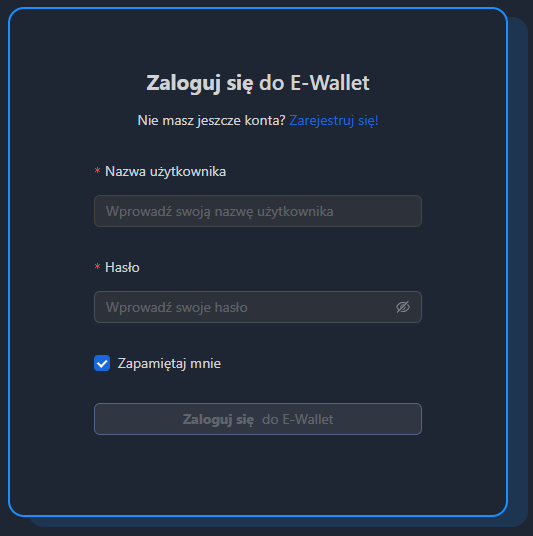
\includegraphics[width=\linewidth]{images/Login}
\end{minipage}
\hfill
\begin{minipage}{0.5\textwidth}
	\centering
	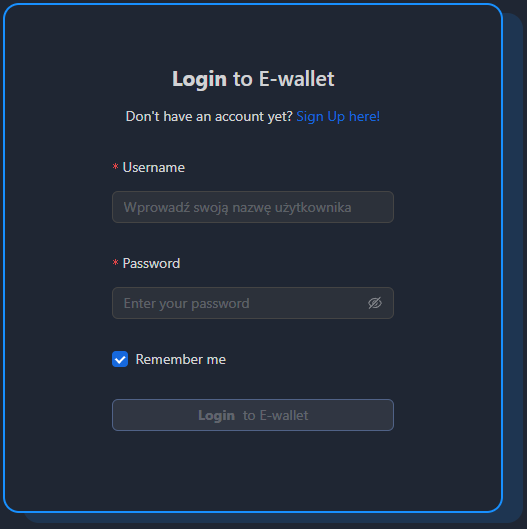
\includegraphics[width=\linewidth]{images/LoginAng}
\end{minipage}
	\caption{Formularz logowania po polsku i angielsku}
	\label{fig:login}
\end{figure}
\begin{figure}[H]
	\centering
	
\includegraphics[width=0.6\linewidth]{images/Navbar}
	\caption{Pasek nawigacyjny}
	\label{fig:navbar}
\end{figure}

\begin{figure}[H]
    \begin{minipage}{0.5\textwidth}
	\centering
	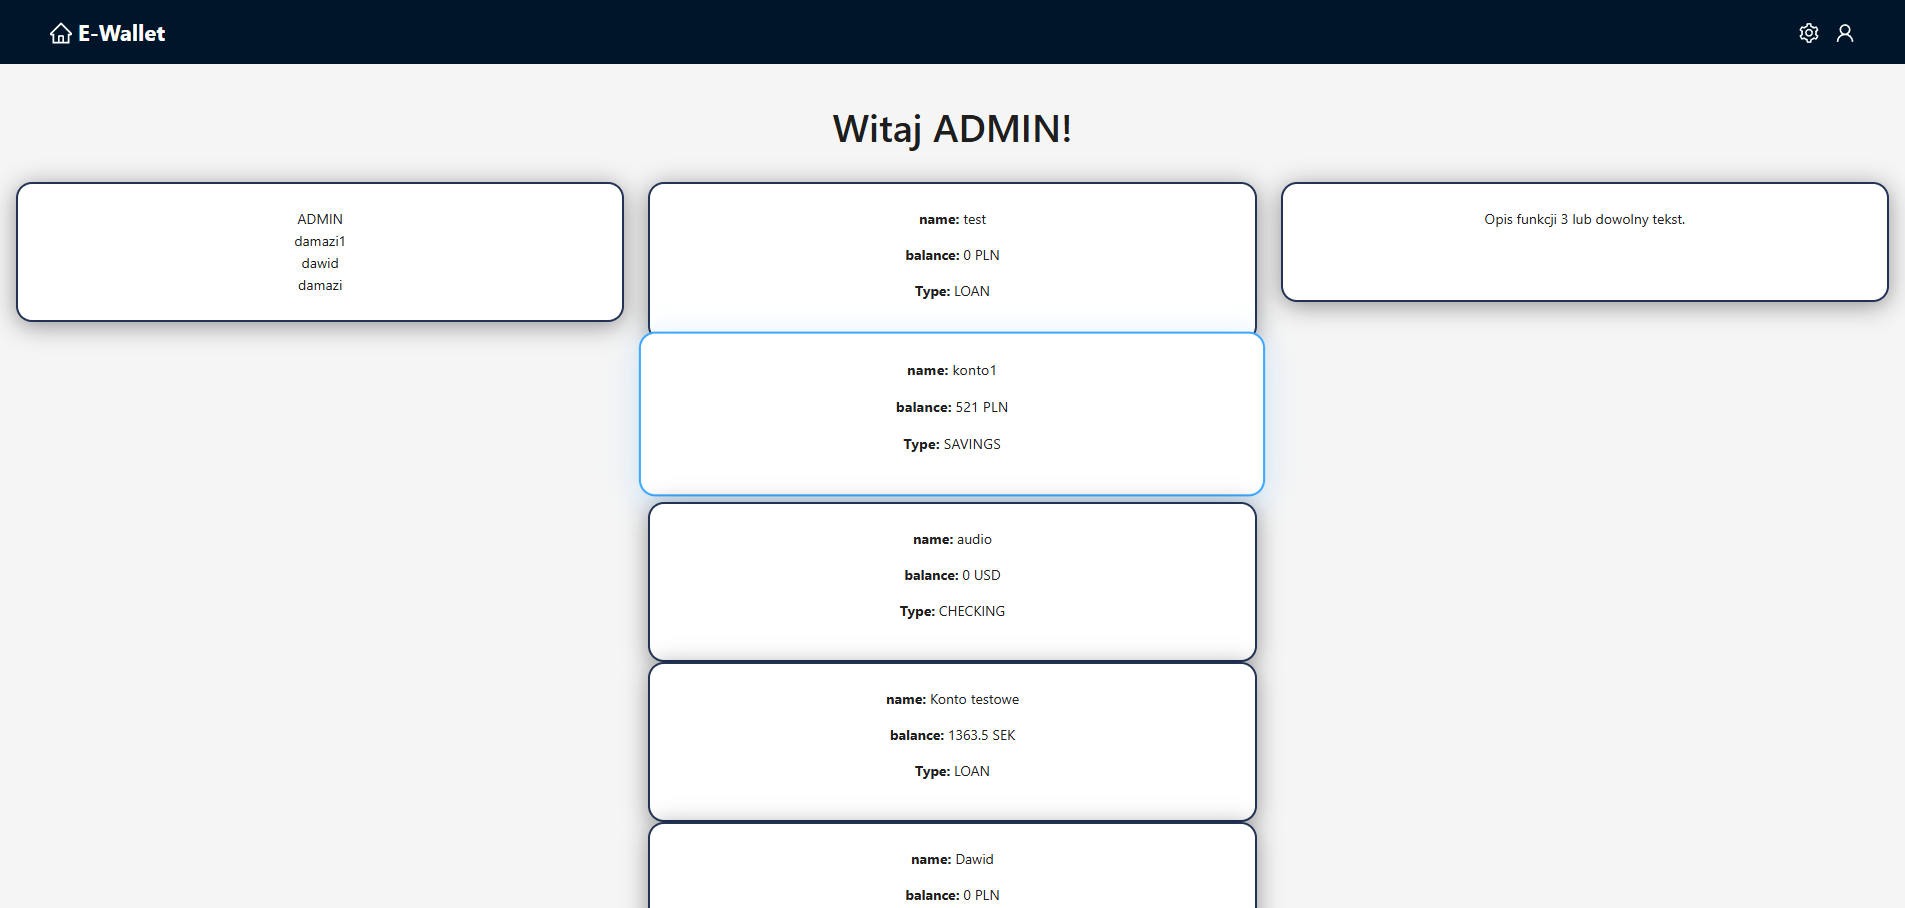
\includegraphics[width=\linewidth]{images/MotywJasny}
\end{minipage}
\hfill
\begin{minipage}{0.5\textwidth}
	\centering
	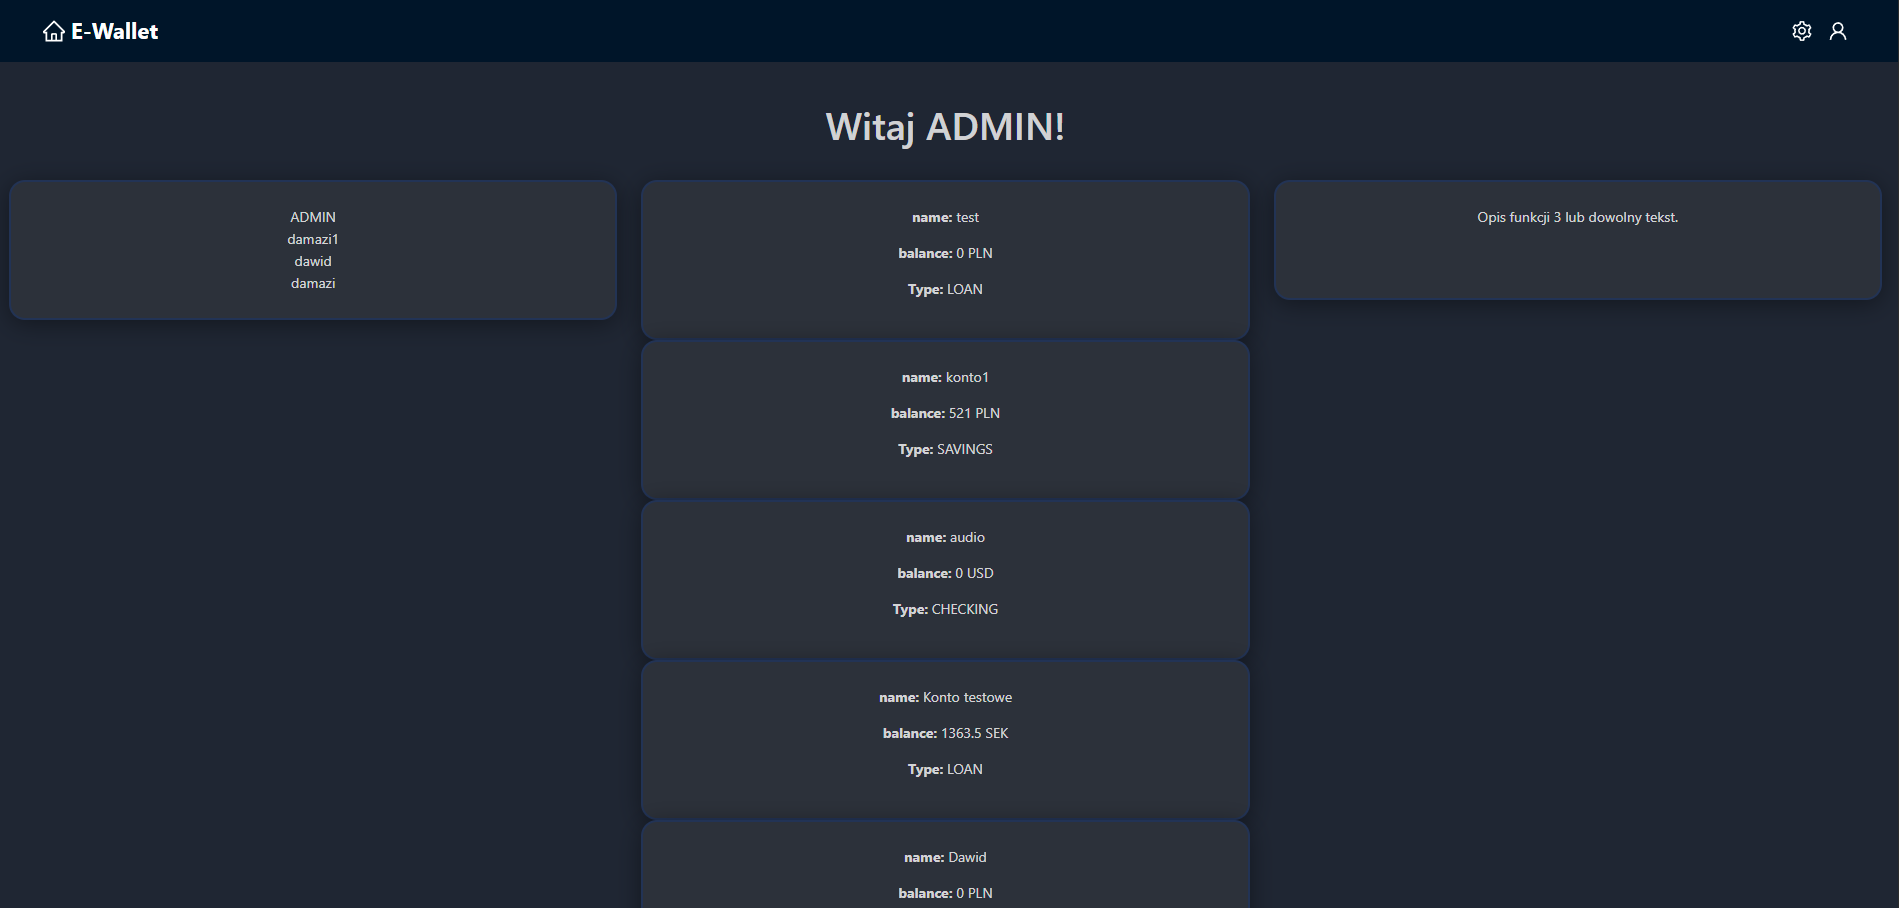
\includegraphics[width=\linewidth]{images/MotywCiemny}
\end{minipage}
	\caption[]{Motywy strony}
	\label{fig:motywy}
\end{figure}

\begin{figure}[H]
	\centering
	
\includegraphics[width=0.7\linewidth]{images/Ustawienia}
	\caption{Ustawienia użytkownika}
	\label{fig:ustawienia}
\end{figure}
\section{Funkcjonalność aplikacji udostępniona użytkownikowi zalogowanemu}
Pomyślna próba logowania spowoduje przekierowanie do strony głównej. System powita użytkownika oraz wypiszę wszystkie portfele aktualnego klienta w postaci kafelków, po których kliknięciu nastąpi przekierowanie do strony danego portfela. Pojawi się również możliwość sprawdzenia szczegółów konta oraz wylogowania po prawej stronie paska nawigacyjnego. 
\subsection*{Szczegóły konta}
Użytkownik może wyświetlić informację o swoim koncie oraz dodać nowe portfele. Dodatkowo jeżeli użytkownik posiada rolę administratora może edytować konta innych użytkowników oraz nadawać uprawnienia.
\\Adres pod którym znajduje się podstrona to \texttt{HOST/details/\{Nazwa\_Użytkownika\}}
\subsection*{Portfel użytkownika}
Klient ma możliwość zarządzania oraz wyświetlania szczegółu na temat portfela. Dane transakcji są przedstawione na wykresach, które umożliwiają wyświetlanie wszystkich transakcji lub podsumowania za każdy dzień (rys. \ref{fig:wykresy}). Użytkownik ma możliwość odczytania informacji o nazwie swojego portfela, ilości dostępnych środków i typie konta. Dostępne są również operację takie jak wpłata, wypłata i przelew (rys. \ref{fig:daneportfela}). Wybranie jednej z operacji otworzy okno modalne wymagające uzupełnienia danych. Ostatnim elementem jest historia wszystkich transakcji, która zawiera kwotę, datę, numer portfela, z którego została wykonana transakcja i numer odbiorcy transakcji oraz status (rys. \ref{fig:transakcjehistoria}). 
\begin{figure}[H]
	\begin{minipage}{0.5\textwidth}
	\centering
	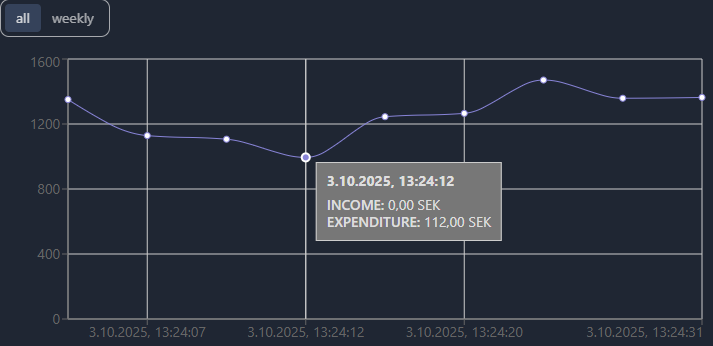
\includegraphics[width=\linewidth]{images/TransakcjeAll}
\end{minipage}
\hfill
\begin{minipage}{0.5\textwidth}
	\centering
	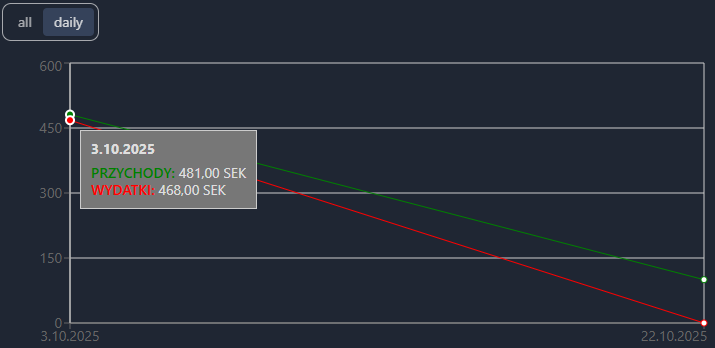
\includegraphics[width=\linewidth]{images/TransakcjeDaily}
\end{minipage}
	\caption{Wykresy wpływów i wypłat z portfela}
	\label{fig:wykresy}
\end{figure}

\begin{figure}[H]
		\begin{minipage}{0.5\textwidth}
	\centering
	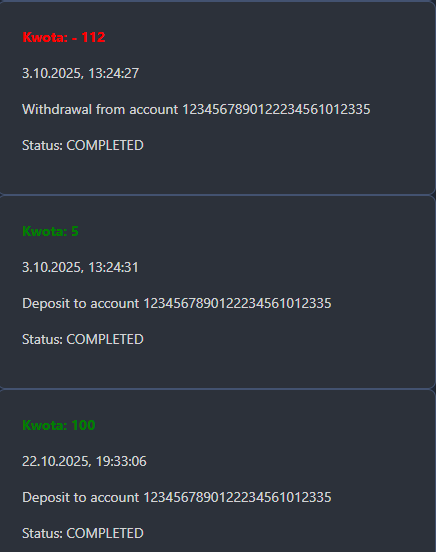
\includegraphics[width=0.7\linewidth]{images/TransakcjeHistoria}
	\caption{Historia transakcji}
	\label{fig:transakcjehistoria}
\end{minipage}
\hfill
		\begin{minipage}{0.5\textwidth}
	\centering
	
\includegraphics[width=\linewidth]{images/DanePortfela}
	\caption{Dane portfela}
	\label{fig:daneportfela}
\end{minipage}
\end{figure}

\chapter{Podsumowanie i wnioski }

Celem niniejszej pracy było zaprojektowanie i implementacja aplikacji webowej wspomagającej zarządzanie finansami. Aplikacja powstała w oparciu o architekturę klient-serwer i posiada takie funkcjonalności jak:
\begin{itemize}
	\item Rejestrowanie i logowanie użytkownika,
	\item Tworzenie różnego rodzaju transakcji,
	\item Sprawdzanie szczegółów profilu lub kont,
	\item Analiza danych finansowych przy pomocy wykresów,
	\item Komunikacja między frontendem, a backendem przy pomocy REST API,
	\item Przechowywanie danych w bazie nierelacyjnej MongoDB.
\end{itemize}
Aplikacja umożliwia elastyczne zarządzanie danymi, dzięki bazie MongoDB. Jej uniwersalny interfejs jest prosty w obsłudze co ułatwia poruszanie się po stronie dla każdej grupy wiekowej. Projekt pozwoli użytkownikowi w łatwiejszy sposób robić takie rzeczy jak:
\begin{itemize}
	\item Zarządzać własnym budżetem domowym,
	\item Śledzić swoje wydatki,
	\item Planować przyszłe płatności,
	\item Wykonywać kroki w celu inwestycji środków.
\end{itemize}
\section*{Wnioski}
Nowoczesne technologie webowe pozwalają na tworzenie skalowalnych i łatwych w rozwoju aplikacji. Architektura klient-serwer sprawdziła się w rozdzieleniu warstwy frontendu od backendu.

W przyszłości aplikację będzie można rozszerzyć o:
\begin{itemize}
	\item Funkcje prognozowania wydatków z wykorzystaniem algorytmów uczenia maszynowego,
	\item Możliwość eksportu danych do formatu PDF lub CSV.
\end{itemize}

Projekt umożliwił rozwinięcie umiejętności analitycznych oraz technicznych związanych z tworzeniem aplikacji webowych.

\section*{Co osiągnąłem}
Podczas realizacji projektu osiągnięto wiele rezultatów. Stworzono kompletną aplikację webową umożliwiającą zarządzanie budżetem domowym, w której połączono wiele nowoczesnych rozwiązań technologicznych. Do najważniejszych osiągnięć należą:
\begin{itemize}
	\item Wykorzystanie architektury klient-serwer,
	\item Interfejs oparty o technologię React,
	\item Opracowanie logiki biznesowej przy pomocy Spring Boot,
	\item Uzyskanie płynnie działającego przepływu danych w bazie MongoDB,
	\item Wdrożenie środowiska do uruchamiania w oparciu o Docker,
	\item Opracowanie testów funkcjonalnych przy użyciu narzędzia Postman,
	\item Umożliwienie dalszej rozbudowy systemu.
\end{itemize}

Realizacja powyższych elementów pozwoliła na stworzenie w pełni działającego systemu, który spełnia założenia projektowe. 

W trakcie tworzenia projektu autor rozwinął swoje umiejętności w zakresie programowania w językach TypeScript i Java, projektowania aplikacji webowych oraz pracy z bazami typu NoSQL. Zdobyte doświadczenie obejmuje również prace z narzędziami takimi jak Git, Docker oraz Postman.

\bibliography{zrodla}

\listoffigures

\listoftables

\lstlistoflistings

\addcontentsline{toc}{chapter}{\lstlistlistingname}
\end{document}
